\documentclass[a4paper, 12pt]{article}
\usepackage{graphicx} % Required for inserting images
\usepackage{fullpage}
\usepackage{amsmath}
\usepackage{xcolor}
\usepackage{float}
\usepackage{geometry}
\usepackage{biblatex}
\geometry{margin=1in}
\usepackage{enumitem}
\usepackage{hyperref}
\usepackage{microtype}
\usepackage{parskip}

\hypersetup{
    colorlinks=true,        % Enable colored links
    linkcolor=teal,         % Set color for internal links
    citecolor=teal,         % Set color for citations
    filecolor=teal,         % Set color for file links
    urlcolor=teal           % Set color for URLs
}

\title{04-20-25 Visually Representing Data}
\author{C\&L Math Tutoring}
\date{April 2025}

\begin{document}

\maketitle

\subsection*{Elements of a plot}

\subsubsection*{Common elements}

\begin{description}
\item [Title] Describes what the plot is about and gives viewers context for what they're looking at.
\item [Axis labels] Tells what each axis represents (with units!).
\item [Legend (or key)] When you have multiple data categories represented by different colors or symbols, the legend tells the viewer what each unique color/symbol represents.
\item [Data points] This is essential! The data points are the core element of a plot.
\end{description}

\subsubsection*{Supplementary elements}

\begin{description}
\item [Regression lines (or lines of best fit)] To show the general direction the data is going in.
\item [Error bars] Little lines that show how much the data might be off, or how confident someone is in their data.
\end{description}

\subsection*{Review of mean, median, and mode}

\begin{description}
\item [Mean] Also known as the average of a dataset. To calculate the mean, add all of the values in the dataset, then divide by the number of values.
\item [Median] The middle number. If there are 2, average them.
\item [Mode] The number that appears most frequently in the dataset. There can be more than one mode.
\end{description}

\subsection*{Line plots}

\begin{figure}[H]
\centering
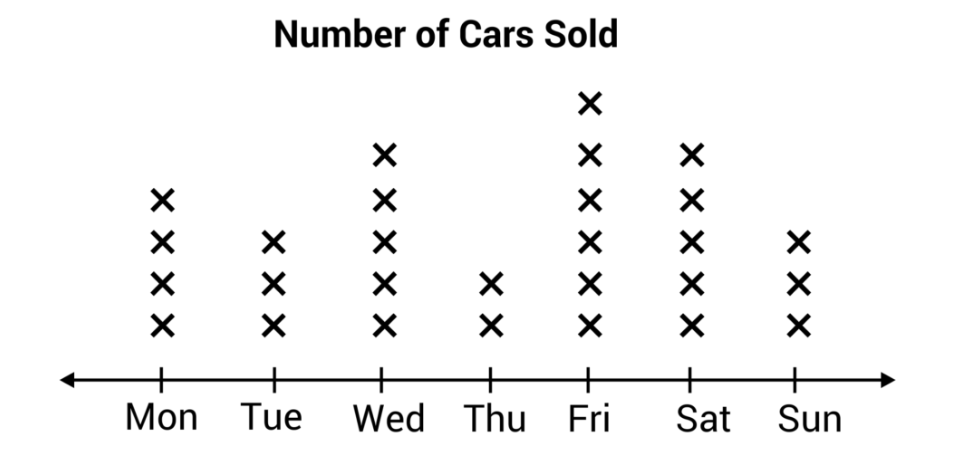
\includegraphics[width=0.6\textwidth]{lineplot}
\end{figure}

This is a line plot representing the number of cars sold on each day of the week. It includes a title, equally spaced tick marks, and the x's aligned well for readability. We assume that each x represents 1 car because whoever created this plot didn't specify otherwise.

To find the median, cross out data points from each end of the line plot until you reach the middle. 

To find the mode, look for the day with the most data points.

\subsection*{Other types of plots}

See \href{https://www.atlassian.com/data/charts/essential-chart-types-for-data-visualization}{this article} for more ways to represent data visually. Some include:

\begin{itemize}
\item scatter plot
\item box plot
\item histogram
\item pie chart
\item density curve
\end{itemize}

\end{document}